\documentclass[tikz,border=12pt]{standalone}
\usepackage{amsmath}
\usepackage{amssymb}
\usepackage{tikz}

\definecolor{ink}{HTML}{0F172A}
\definecolor{linegray}{HTML}{64748B}
\definecolor{visible}{HTML}{E2E8F0}
\definecolor{masked}{HTML}{F8FAFC}
\definecolor{maskedge}{HTML}{94A3B8}
\definecolor{prediction}{HTML}{F1F5F9}
\definecolor{lossfill}{HTML}{CBD5E1}

\begin{document}
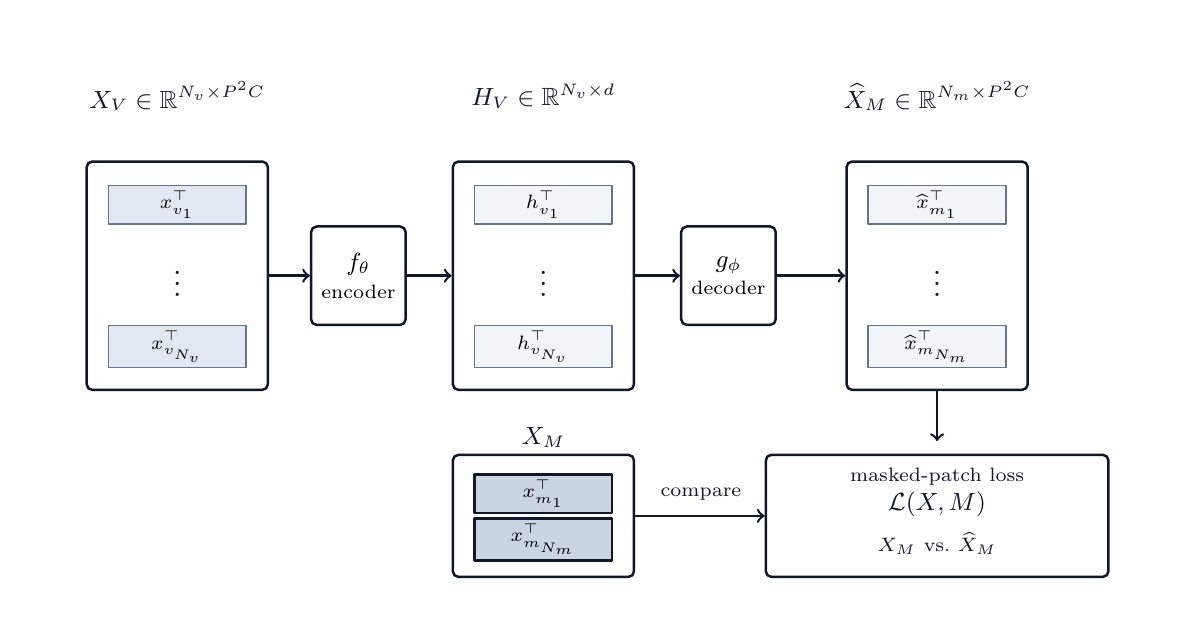
\begin{tikzpicture}[
  font=\sffamily,
  line cap=round,
  line join=round,
  panel/.style={
    draw=ink,
    line width=0.9pt,
    rounded corners=2pt,
    minimum width=2.3cm,
    minimum height=2.9cm,
    inner sep=0pt
  },
  small panel/.style={
    panel,
    minimum height=1.55cm
  },
  module/.style={
    draw=ink,
    line width=0.9pt,
    rounded corners=2pt,
    minimum width=1.2cm,
    minimum height=1.25cm,
    inner sep=3pt,
    align=center,
    font=\small
  },
  row/.style={
    draw=linegray,
    line width=0.6pt,
    minimum width=1.75cm,
    minimum height=0.42cm,
    inner sep=2pt,
    align=center,
    font=\scriptsize
  },
  masked row/.style={
    row,
    draw=maskedge,
    dashed,
    fill=masked
  },
  prediction row/.style={
    row,
    fill=prediction
  },
  loss row/.style={
    row,
    draw=ink,
    line width=0.8pt,
    fill=lossfill
  }
]
  \fill[white] (-0.55,-2.0) rectangle (13.75,5.35);

  % Visible tokens entering the encoder.
  \node[panel] (input) at (1.35,2.2) {};
  \node[ink, font=\small] at (1.35,4.48)
    {$X_V \in \mathbb{R}^{N_v\times P^2 C}$};
  \node[row, fill=visible] at (1.35,3.1) {$x_{v_1}^{\top}$};
  \node[ink, font=\large] at (1.35,2.2) {$\vdots$};
  \node[row, fill=visible] at (1.35,1.3) {$x_{v_{N_v}}^{\top}$};

  % Encoder representation.
  \node[module] (encoder) at (3.65,2.2) {$f_\theta$\\[-1pt]\scriptsize encoder};
  \node[panel] (latent) at (6.0,2.2) {};
  \node[ink, font=\small] at (6.0,4.48)
    {$H_V \in \mathbb{R}^{N_v\times d}$};
  \node[row, fill=prediction] at (6.0,3.1) {$h_{v_1}^{\top}$};
  \node[ink, font=\large] at (6.0,2.2) {$\vdots$};
  \node[row, fill=prediction] at (6.0,1.3) {$h_{v_{N_v}}^{\top}$};

  % Decoder reconstruction.
  \node[module] (decoder) at (8.35,2.2) {$g_\phi$\\[-1pt]\scriptsize decoder};
  \node[panel] (output) at (11.0,2.2) {};
  \node[ink, font=\small] at (11.0,4.48)
    {$\widehat{X}_M \in \mathbb{R}^{N_m\times P^2 C}$};
  \node[row, fill=prediction] at (11.0,3.1) {$\widehat{x}_{m_1}^{\top}$};
  \node[ink, font=\large] at (11.0,2.2) {$\vdots$};
  \node[row, fill=prediction] at (11.0,1.3) {$\widehat{x}_{m_{N_m}}^{\top}$};

  % The forward path.
  \draw[ink, ->, line width=0.9pt] (input.east) -- (encoder.west);
  \draw[ink, ->, line width=0.9pt] (encoder.east) -- (latent.west);
  \draw[ink, ->, line width=0.9pt] (latent.east) -- (decoder.west);
  \draw[ink, ->, line width=0.9pt] (decoder.east) -- (output.west);

  % Original masked targets and the training loss.
  \node[small panel] (target) at (6.0,-0.85) {};
  \node[ink, font=\small] at (6.0,0.15) {$X_M$};
  \node[loss row] at (6.0,-0.57) {$x_{m_1}^{\top}$};
  \node[ink, font=\scriptsize] at (6.0,-0.86) {$\vdots$};
  \node[loss row] at (6.0,-1.15) {$x_{m_{N_m}}^{\top}$};

  \node[small panel, minimum width=4.35cm] (loss) at (11.0,-0.85) {};
  \node[ink, font=\scriptsize] at (11.0,-0.35) {masked-patch loss};
  \node[ink, font=\small] at (11.0,-0.7) {$\mathcal{L}(X,M)$};
  \node[ink, font=\scriptsize] at (11.0,-1.2)
    {$X_M\ \text{vs.}\ \widehat{X}_M$};

  \draw[ink, ->, line width=0.9pt] (output.south) -- (11.0,0.1);
  \draw[ink, ->, line width=0.9pt] (target.east) -- (loss.west);
  \node[ink, font=\scriptsize, fill=white, inner sep=1pt]
    at (8.0,-0.58) {compare};
\end{tikzpicture}
\end{document}
